% Fundamentos Matemáticos para Computação 1 - 2015.2
% Avaliação 2: Teoria dos Números, Congruência
% Autor: Patrick Terrematte

\documentclass[11pt,a4paper]{article}
%\usepackage[latin1]{inputenc}   % Descomentar para compilar no windows
\usepackage[utf8x]{inputenc}     % Comentar para compilar no windows
\usepackage{graphicx}
\usepackage{svg}
\usepackage{color}
\usepackage{xspace}
%\usepackage[brazil]{babel}
%\usepackage[latin1]{inputenc}
\usepackage{amsfonts, amssymb,amsmath}
\usepackage{array,booktabs}
\usepackage{proof}
\usepackage{fancyhdr}
 \usepackage{paralist}
%\usepackage[pdftex=true,pagebackref=true,bookmarks=true,bookmarksnumbered=true,pdffitwindow=true]{hyperref}
\usepackage{hyperref}
\usepackage{marginnote}
%\usepackage[top=Bcm, bottom=Hcm, outer=Ccm, inner=Acm, heightrounded, marginparwidth=Ecm, marginparsep=Dcm]{geometry}
\usepackage{comment}
\usepackage{tkz-euclide}
\usepackage{multicol}
\usepackage[export]{adjustbox}

\renewcommand{\b}{\textbf}
\newcommand{\noi}{\noindent}
\newcommand{\Z}{\mathbb{Z}}
\newcommand{\N}{\mathbb{N}}

\setlength{\textwidth}{170mm}%
\setlength{\textheight}{279mm}%
\setlength{\topmargin}{-20mm}%
%\setlength{\bottommargin}{}%
\setlength{\oddsidemargin}{-10mm}
\setlength{\evensidemargin}{-30mm}%

\begin{document}
\frenchspacing
\begin{center}
    \begin{minipage}{4cm}
		\begin{center}
			\includegraphics[width=4cm, height=2.0cm]{logoifb.jpeg}
		\end{center}
	\end{minipage}
	\begin{minipage}{11.4cm}
		\begin{center}
				{\small \textsc{Instituto Federal de Brasília}			\\
						  \textsc{Campus Samambaia}\\
						  \textsc{3º ano - Ensino Médio Integrado} \\
                          \textsc{\textbf{Professor:} Bruno Xavier}\\
                }
		\end{center}
	\end{minipage}
	%\begin{minipage}{1.6cm}
	%	\begin{center}
	%		\includegraphics[width=2cm, height=1.1cm]{logoimd.png}
	%	\end{center}
	%\end{minipage}
\end{center}


{\sf
  \begin{center}
    \Large \textbf{--- Folha de Respostas ---}%
  \end{center}
}\bigskip

\setlength{\marginparwidth}{5cm}
\small \noindent \textbf{Nome:}\hspace{0.3cm} HEADNOME
\hrulefill \hspace{0.1cm}
\textbf{Matricula:}\hspace{0.1cm} HEADMATRICULA \\*[0.1cm]
\textbf{Bimestre:}\hspace{0.1cm} 1° \\*[0.1cm]

\vspace{5cm}
\begin{center}
%\framebox{%
%  \begin{minipage}{0.6\linewidth}
{\Huge \hspace{0pt}$\blacksquare$\hspace{-4pt}$\blacksquare$}\hspace{350pt}{\Huge $\blacksquare$\hspace{-4pt}$\blacksquare$} \\
\begin{minipage}{0.3\textwidth}
\begin{center}
%\begin{figure}[h!]
%	\centering
	\includegraphics[width=0.8\textwidth]{QRMATRICULA}
%\end{figure}
%This is the first column.
%This is still in the first column. \\
\end{center}
\end{minipage}
%second column
\begin{minipage}{0.45\textwidth}
\begin{center}
\begin{tikzpicture}[font=\small]
	\foreach \count/\desc in {1/A, 2/B, 3/C, 4/D, 5/E} { 
                \node at ({\count}, 0.4) {};
                \node at (0,0) {\smallsize{\tiny Tipo \quad}};
                \node[draw,circle,very thick,inner sep=3pt] at ({\count},0) {\tiny \desc};
            }
    \foreach \line in {1,2,...,10} {
        \begin{scope}[yshift=-\line cm]
            \foreach \count/\desc in {1/A, 2/B, 3/C, 4/D, 5/E} { 
                \node at ({\count}, 0.4) {};
                \node at (0,0) {\smallsize{\tiny \line \quad}};
                \node[draw,circle,very thick,inner sep=3pt] at ({\count},0) {\tiny \desc};
            }
        \end{scope}
    }
\end{tikzpicture}
\end{center}
\end{minipage} \\
\null{\Huge \hspace{0pt}$\blacksquare$\hspace{-4pt}$\blacksquare$}\hspace{350pt}{\Huge $\blacksquare$\hspace{-4pt}$\blacksquare$}
  %\end{minipage}}
 \end{center}
\end{document}
